% Slide bao ve luan van thac si -- mau HUST PPT template 2022 (anh nen, logo, mau do, font Lato
% lay tu mau chinh thuc tai hust.edu.vn, thu muc hust/).
% Bien dich: xelatex defense_slides.tex (2 lan). Hinh TikZ lay tu luan van: python extract_figures.py
\documentclass[aspectratio=169,10pt,t]{beamer}
\usepackage{fontspec}
\setsansfont{Lato}[Extension=.ttf, UprightFont=*-Regular, BoldFont=*-Bold,
                   ItalicFont=*-Italic, BoldItalicFont=*-BoldItalic]
\usepackage{amsmath, amssymb, bm}
\usefonttheme{professionalfonts}
\usepackage{booktabs}
\usepackage{tikz}
\usetikzlibrary{calc, positioning, arrows.meta}
\graphicspath{{hust/}{figures/}{../thesis/figures/}}
%% Khung bao (pt) cua so do day du, do extract_figures.py ghi ra
\def\mapSWx{-12.98091}
\def\mapSWy{-430.07796}
\def\mapNEx{586.5267}
\def\mapNEy{61.25139}
\def\mapBorder{2}


% ---------- Mau va ky hieu ----------
\definecolor{hustred}{HTML}{CD1628}
\definecolor{ink}{HTML}{262626}
\definecolor{muted}{HTML}{6E6E6E}
\definecolor{tint}{HTML}{FCEEEF}
\definecolor{linegray}{HTML}{D9D9D9}
\newcommand{\R}{\mathbb{R}}
\newcommand{\T}{\mathsf{T}}
\DeclareMathOperator{\sig}{sig}
\DeclareMathOperator{\Proj}{Proj}
\DeclareMathOperator{\diag}{diag}

% ---------- Giao dien theo mau HUST ----------
\setbeamertemplate{navigation symbols}{}
\setbeamersize{text margin left=0.65cm, text margin right=0.65cm}
\setbeamercolor{normal text}{fg=ink}
\setbeamercolor{structure}{fg=hustred}
\setbeamercolor{alerted text}{fg=hustred}
\setbeamerfont{frametitle}{size=\Large, series=\bfseries}
\setbeamercolor{frametitle}{fg=hustred}
\setbeamertemplate{itemize item}{\raisebox{0.12ex}{\color{hustred}\scriptsize$\blacktriangleright$}}
\setbeamertemplate{itemize subitem}{\color{hustred}\textendash}
\setbeamertemplate{enumerate item}{\color{hustred}\bfseries\insertenumlabel.}
\setlength{\leftmargini}{1.1em}
\setbeamertemplate{background}{
\includegraphics[width=\paperwidth,height=\paperheight]{bg_content.jpg}}
\setbeamertemplate{frametitle}{%
  \vspace*{0.28cm}%
  \ifnum\value{section}>0{\scriptsize\color{muted}\insertsectionnumber.~\insertsection\par}\vspace{0.04cm}\fi
  {\usebeamerfont{frametitle}\usebeamercolor[fg]{frametitle}\insertframetitle\par}%
  \vspace*{0.05cm}}
\setbeamertemplate{footline}{%
  \begin{tikzpicture}[remember picture, overlay]
    \node[anchor=east, text=white, font=\scriptsize\bfseries]
      at ($(current page.south east)+(-0.5cm,0.36cm)$) {\insertframenumber};
  \end{tikzpicture}}

% Khoi noi bat va the
\tikzset{
  card/.style={fill=tint, rounded corners=4pt, inner sep=6pt, align=left},
  hl/.style={draw=hustred, line width=1.3pt, fill=hustred, fill opacity=0.2, rounded corners=2pt},
}
\newcommand{\stat}[2]{% so lon + chu thich
  {\fontsize{20}{22}\selectfont\bfseries\color{hustred}#1}\\[1pt]{\footnotesize #2}}
\newcommand{\hint}[1]{{\footnotesize\color{muted}#1}}

% Ban do thu nho cua so do day du (Hinh 4.2 cua luan van) o goc tren phai, #1: cac khoi to sang
% ve theo toa do cua chinh hinh do (cm).
\newlength{\mmW}\setlength{\mmW}{3.9cm}
\newcommand{\minimap}[1]{%
  \begin{tikzpicture}[remember picture, overlay]
    \node[anchor=north east, inner sep=2pt, draw=linegray, fill=white, rounded corners=2pt] (mm)
      at ($(current page.north east)+(-0.35cm,-0.28cm)$) {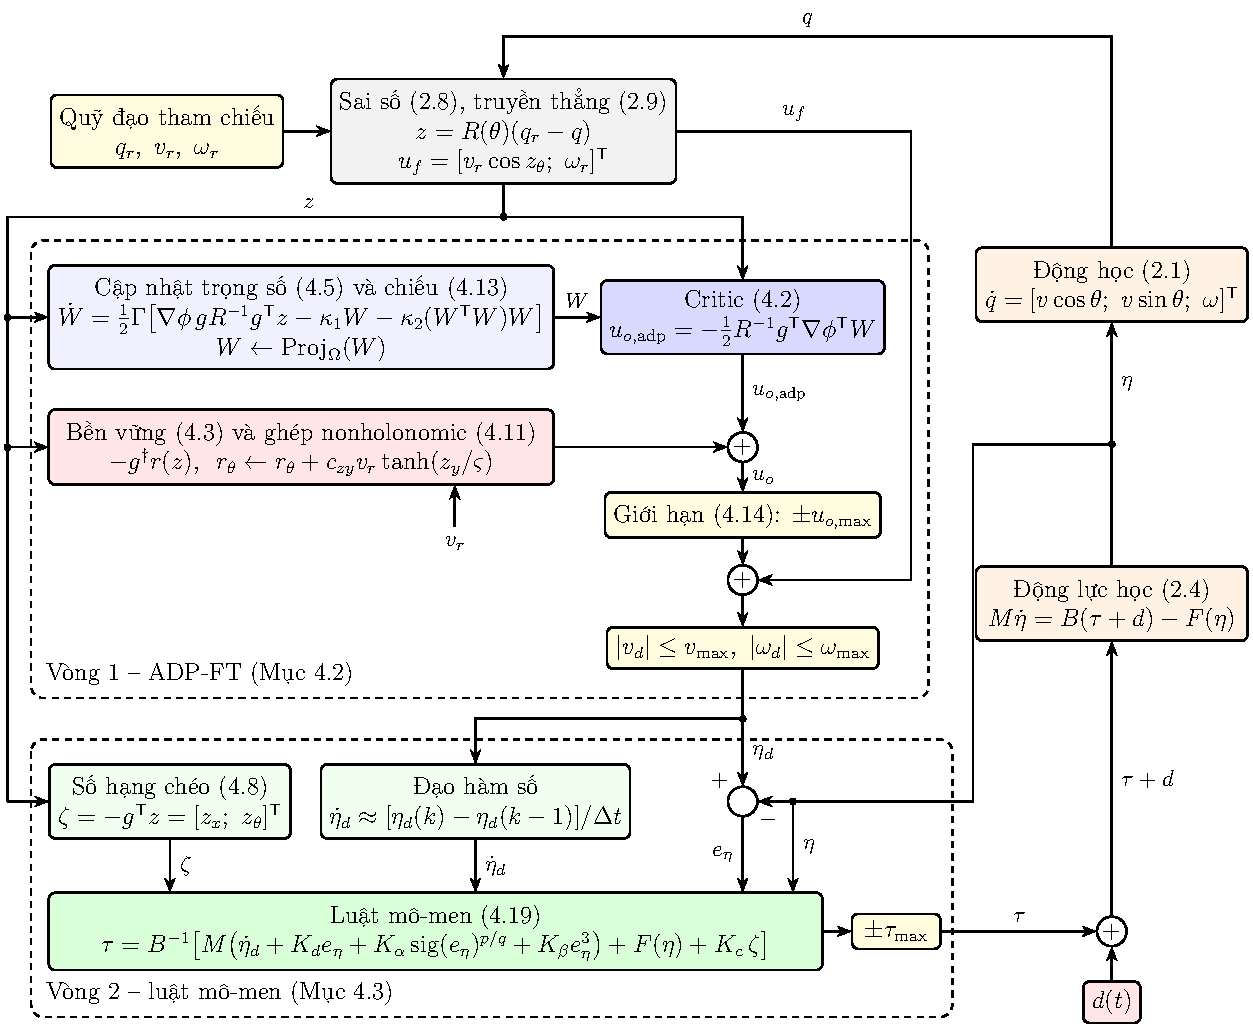
\includegraphics[width=\mmW]{controller_full.pdf}};
    \pgfmathsetmacro{\mms}{\mmW/(\mapNEx-\mapSWx+2*\mapBorder)}
    \begin{scope}[shift={($(mm.south west)+(2pt,2pt)+({\mapBorder*\mms*1pt},{\mapBorder*\mms*1pt})$)}]
      \begin{scope}[scale=\mms]
        \begin{scope}[shift={({-1*(\mapSWx)*1pt},{-1*(\mapSWy)*1pt})}]
          #1
        \end{scope}
      \end{scope}
    \end{scope}
    \node[anchor=north east, font=\tiny, text=muted, inner sep=1pt] at ($(mm.south east)+(0,-0.04cm)$) {vị trí trên sơ đồ đầy đủ};
  \end{tikzpicture}}
% Vung cac khoi tren so do day du (toa do cm cua hinh)
\newcommand{\hlLoopOne}{\path[hl] (-0.1,-1.75) rectangle (15.3,-9.7);}
\newcommand{\hlLoopTwo}{\path[hl] (-0.1,-10.2) rectangle (15.7,-15.1);}
\newcommand{\hlRobust}{\path[hl] (0.15,-6.25) rectangle (9.0,-4.45);}
\newcommand{\hlCross}{\path[hl] (0.15,-12.25) rectangle (4.55,-10.45); \path[hl] (0.15,-14.45) rectangle (13.55,-12.65);}

\title{Ứng dụng điều khiển ADP cho xe tự hành}
\author{Nguyễn Thành Trung}

\begin{document}

% ================================================================ Bia
{\setbeamertemplate{background}{
\includegraphics[width=\paperwidth,height=\paperheight]{bg_title.jpg}}
\begin{frame}[plain]
\begin{tikzpicture}[remember picture, overlay]
  \node[anchor=north west, inner sep=0] at ($(current page.north west)+(0.5cm,-0.45cm)$)
    {
\includegraphics[width=4.3cm]{logo_lockup.png}};
  \node[anchor=north west, inner sep=0, text width=12cm, align=left]
    at ($(current page.north west)+(0.65cm,-2.35cm)$) {%
    {\footnotesize\bfseries\color{muted}TRƯỜNG ĐIỆN -- ĐIỆN TỬ\quad\textbullet\quad LUẬN VĂN THẠC SĨ}\\[0.32cm]
    {\fontsize{22}{27}\selectfont\bfseries\color{hustred}ỨNG DỤNG ĐIỀU KHIỂN ADP\\CHO XE TỰ HÀNH}\\[0.42cm]
    {\small Ngành: Kỹ thuật Điều khiển và Tự động hóa}\\[0.45cm]
    {\small\bfseries Học viên: Nguyễn Thành Trung}\\[0.1cm]
    {\small Giáo viên hướng dẫn: PGS.TS. Nguyễn Hoài Nam}\\[0.42cm]
    {\footnotesize\color{muted}Hà Nội, 2026}};
\end{tikzpicture}
\end{frame}}

% ================================================================ Noi dung
\newcommand{\agenda}[3]{%
  \begin{tikzpicture}[baseline=(c.base)]
    \node[circle, fill=hustred, text=white, font=\small\bfseries, minimum size=0.62cm, inner sep=0] (c) {#1};
  \end{tikzpicture}\hspace{0.32cm}%
  \begin{minipage}[c]{9.8cm}{\bfseries #2}\\[1pt]{\footnotesize\color{muted}#3}\end{minipage}\par\vspace{0.26cm}}
\begin{frame}{Nội dung trình bày}
  \vspace{0.15cm}
  \agenda{1}{Đặt vấn đề}{Bối cảnh, khoảng trống, mục tiêu và đóng góp}
  \agenda{2}{Mô hình robot và sai số bám}{Mô hình 5 trạng thái nhận mô-men; sai số trong hệ tọa độ thân robot}
  \agenda{3}{Bộ điều khiển hai vòng theo backstepping}{Vòng 1 ADP-FT, khoảng hở kênh ngang và số hạng ghép, vòng 2, Định lý 4.1}
  \agenda{4}{Kết quả mô phỏng}{Bám quỹ đạo, so sánh năm phương pháp, độ bền với nhiễu}
  \agenda{5}{Kết luận}{Đóng góp, hạn chế và hướng phát triển}
\end{frame}

% ================================================================ 1. Dat van de
\section{Đặt vấn đề}
\begin{frame}{Bối cảnh và khoảng trống}
  \begin{columns}[T,onlytextwidth]
    \begin{column}{0.33\textwidth}
      \vspace{0.1cm}
      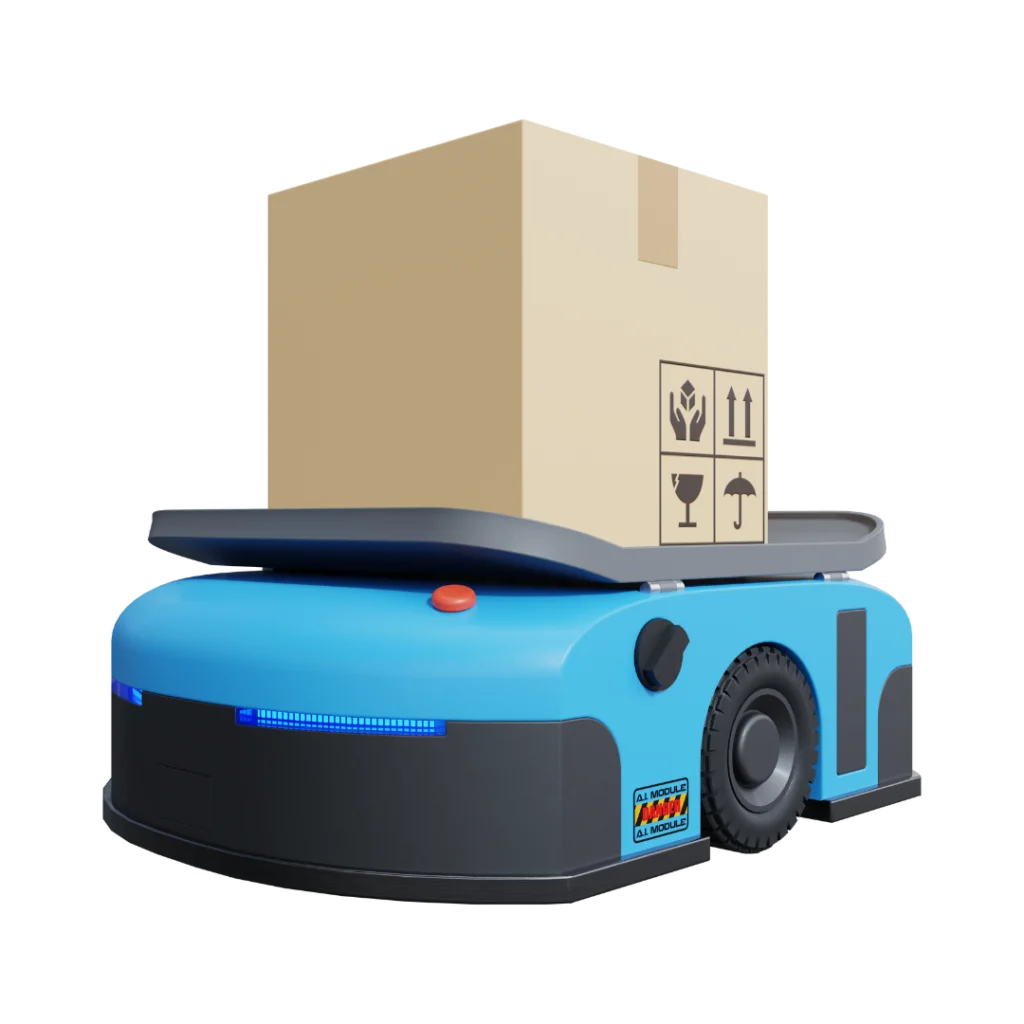
\includegraphics[width=\linewidth]{agv_example.png}\\[2pt]
      \hint{Robot tự hành vận chuyển hàng trong nhà máy}
    \end{column}
    \begin{column}{0.63\textwidth}
      \begin{itemize}\setlength{\itemsep}{0.32cm}
        \item \textbf{Bài toán:} robot vi sai bám quỹ đạo tham chiếu $q_r(t)$ -- sai số về nhỏ nhanh, tốn ít năng lượng điều khiển.
        \item \textbf{Hướng ADP hội tụ cố định thời gian} (Wang et al., IEEE RA-L 2025): luật vận tốc gần tối ưu, sai số vào lân cận gốc trong thời gian bị chặn, không cần tín hiệu kích thích liên tục.
        \item \textbf{Khoảng trống:} luật chỉ xét \alert{mô hình động học} -- đầu vào là vận tốc $(v,\omega)$. Robot thực nhận \alert{mô-men} hai bánh, có quán tính, ma sát, giới hạn mô-men và nhiễu.
      \end{itemize}
    \end{column}
  \end{columns}
\end{frame}

\begin{frame}{Mục tiêu và đóng góp}
  {\small\textbf{Mục tiêu:} thiết kế bộ điều khiển \textbf{hai vòng theo backstepping} cho robot nhận lệnh mô-men, với vòng 1 là luật ADP hội tụ cố định thời gian (ADP-FT).\par}
  \vspace{0.3cm}
  \begin{tikzpicture}[every node/.style={card, anchor=north west, text width=6.4cm, minimum height=1.5cm}]
    \node (c1) at (0,0)
      {{\bfseries\color{hustred}1\enspace Vòng 2 theo backstepping}\\[2pt]{\footnotesize Luật mô-men có số hạng chéo; Định lý 4.1: vòng 2 không làm hỏng vòng 1.}};
    \node (c2) at (7.45,0)
      {{\bfseries\color{hustred}2\enspace Khoảng hở kênh ngang}\\[2pt]{\footnotesize Bổ đề 4.1: luật gốc không tác động được lên $z_y$; khắc phục bằng số hạng ghép.}};
    \node (c3) at ($(c1.south west)+(0,-0.22)$)
      {{\bfseries\color{hustred}3\enspace So sánh công bằng}\\[2pt]{\footnotesize Năm phương pháp, cùng vòng 2, cùng quy trình chỉnh hệ số, ba quỹ đạo.}};
    \node (c4) at ($(c2.south west)+(0,-0.22)$)
      {{\bfseries\color{hustred}4\enspace Độ bền và vai trò thành phần}\\[2pt]{\footnotesize Nhiễu mô-men ba dạng tới $60\%\,\tau_{\max}$; thí nghiệm bỏ từng thành phần.}};
  \end{tikzpicture}
\end{frame}

% ================================================================ 2. Mo hinh
\section{Mô hình robot và sai số bám}
\begin{frame}{Mô hình robot vi sai 5 trạng thái}
  \begin{columns}[T,onlytextwidth]
    \begin{column}{0.44\textwidth}
      \vspace{0.05cm}
      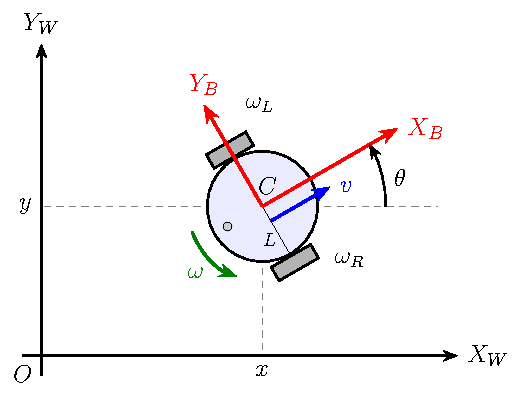
\includegraphics[width=\linewidth]{wmr_schematic.pdf}
    \end{column}
    \begin{column}{0.53\textwidth}
      \small
      \[
        \left\{
        \begin{aligned}
          \dot x &= v\cos\theta, \quad \dot y = v\sin\theta, \quad \dot\theta = \omega\\
          \dot v &= \frac{1}{m}\Big(\frac{\tau_R + \tau_L}{r} - f_v v - f_c\tanh\frac{v}{\varepsilon}\Big)\\
          \dot\omega &= \frac{1}{I}\Big(\frac{L(\tau_R - \tau_L)}{r} - f_\omega\omega - f_{c\omega}\tanh\frac{\omega}{\varepsilon}\Big)
        \end{aligned}
        \right.
      \]
      \begin{itemize}\setlength{\itemsep}{0.12cm}
        \item Ba phương trình đầu: \textbf{động học}; hai phương trình cuối: \textbf{động lực học} $M\dot\eta = B\tau - F(\eta)$ (Fierro \& Lewis).
        \item Đầu vào thật là \alert{mô-men} $\tau = [\tau_R, \tau_L]^\T$, bị chặn $|\tau_i| \le 1$\,N$\cdot$m.
      \end{itemize}
    \end{column}
  \end{columns}
\end{frame}

\begin{frame}{Sai số bám trong hệ tọa độ thân robot}
  \begin{columns}[T,onlytextwidth]
    \begin{column}{0.42\textwidth}
      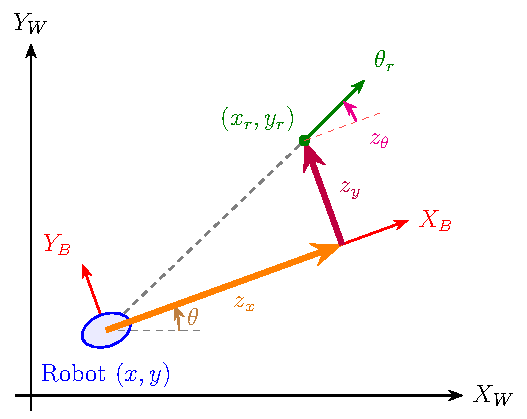
\includegraphics[width=\linewidth]{error_body_frame.pdf}
    \end{column}
    \begin{column}{0.55\textwidth}
      \small
      \[ z = \begin{bmatrix} z_x \\ z_y \\ z_\theta \end{bmatrix} = R(\theta)\,(q_r - q), \qquad u = u_f + u_o \]
      \[ \dot z = f(z, u_r) + g(z)\,u_o, \qquad g(z) = \begin{bmatrix} -1 & z_y \\ 0 & -z_x \\ 0 & -1 \end{bmatrix} \]
      \begin{itemize}\setlength{\itemsep}{0.1cm}
        \item $u_f = [v_r\cos z_\theta;\ \omega_r]$: phần truyền thẳng.
        \item $u_o$: phần phản hồi do bộ điều khiển thiết kế.
        \item Hàng thứ hai của $g$: $u_o$ chỉ tác động gián tiếp lên \alert{sai số ngang $z_y$} (nonholonomic).
      \end{itemize}
    \end{column}
  \end{columns}
\end{frame}

% ================================================================ 3. Bo dieu khien
\section{Bộ điều khiển hai vòng theo backstepping}
\begin{frame}{Cấu trúc hai vòng}
  \begin{tikzpicture}[remember picture, overlay]
    \node[anchor=north west, inner sep=0] (fig) at ($(current page.north west)+(0.65cm,-1.45cm)$)
      {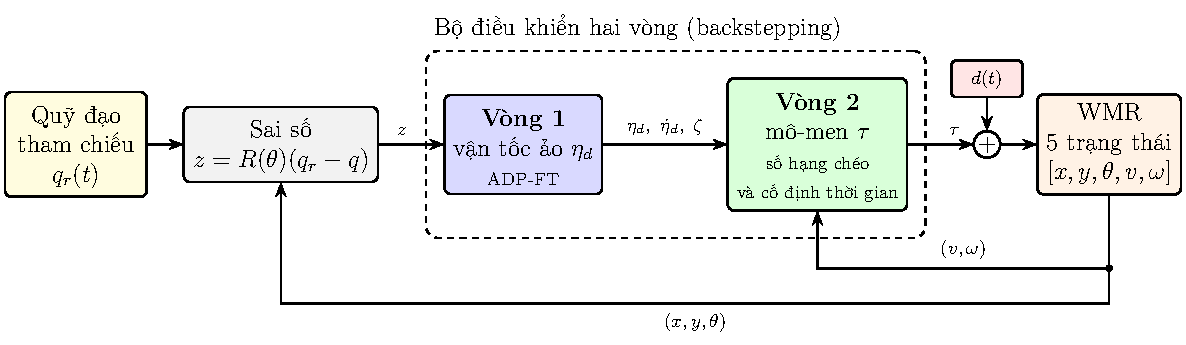
\includegraphics[width=14.6cm]{architecture.pdf}};
    \node[card, anchor=north west, text width=4.7cm] (a) at ($(fig.south west)+(0,-0.3cm)$)
      {{\bfseries\color{hustred}Vòng 1 -- vòng ngoài}\\[1pt]{\footnotesize Chọn vận tốc ảo $\eta_d$ từ sai số $z$: luật ADP-FT.}};
    \node[card, anchor=north west, text width=4.7cm] at ($(a.north east)+(0.3cm,0)$)
      {{\bfseries\color{hustred}Vòng 2 -- vòng trong}\\[1pt]{\footnotesize Chọn mô-men $\tau$ để $\eta \to \eta_d$; suy từ hàm Lyapunov của vòng 1.}};
  \end{tikzpicture}
\end{frame}

\begin{frame}{Sơ đồ đầy đủ của bộ điều khiển}
  \begin{tikzpicture}[remember picture, overlay]
    \node[anchor=north west, inner sep=0] at ($(current page.north west)+(0.65cm,-1.3cm)$)
      {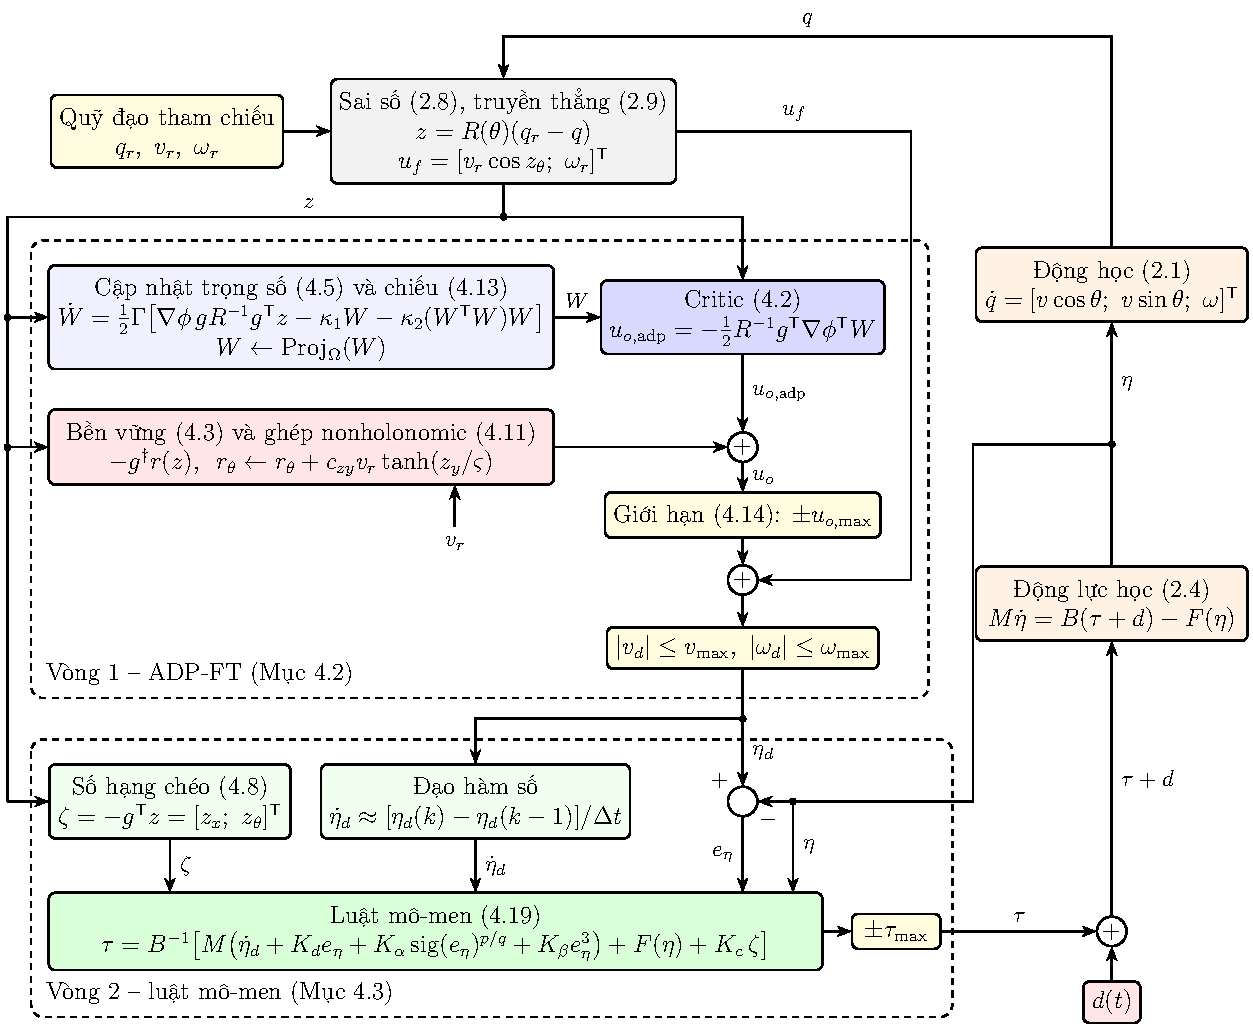
\includegraphics[height=6.75cm]{controller_full.pdf}};
    \node[anchor=north west, text width=5.9cm, align=left] at ($(current page.north west)+(9.25cm,-1.65cm)$) {%
      \small
      {\bfseries\color{hustred}Cách đọc}\\[3pt]
      \footnotesize
      \textbf{Khung trên}: vòng 1 -- ADP-FT (Mục 4.2)\\[2pt]
      \textbf{Khung dưới}: vòng 2 -- luật mô-men (Mục 4.3)\\[2pt]
      \textbf{Cột phải}: robot (Chương 2)\\[8pt]
      {\bfseries\color{hustred}Mỗi chu kỳ lấy mẫu 1\,ms}\\[3pt]
      1.\ đo $q$, $\eta$ $\to$ tính $z$, $u_f$\\[1pt]
      2.\ vòng 1 tính $\eta_d$ với trọng số $W$ hiện tại\\[1pt]
      3.\ cập nhật $W$ và chiếu về tập $\Omega$\\[1pt]
      4.\ vòng 2 tính $\tau$, bão hòa ở $\pm\tau_{\max}$};
  \end{tikzpicture}
\end{frame}

\begin{frame}{Vòng 1: luật ADP-FT}
  \minimap{\hlLoopOne}
  \begin{minipage}[t]{10.6cm}
  \small
  \vspace{0.05cm}
  \[ u_o = u_{o,\text{adp}} - g^\dagger(z)\,r(z), \qquad u_{o,\text{adp}} = -\tfrac12 R^{-1} g^\T \nabla\phi^\T W \]
  \hint{Thành phần gần tối ưu từ mạng Critic (hàm giá trị $\hat V = W^\T\phi(z)$, $\phi$: 6 đơn thức bậc hai của $z$) và thành phần bền vững.}
  \[ r(z) = \bm\lambda\odot\tanh\tfrac{z}{\rho} + \bm\mu\odot z + \bm\alpha\odot\sig(z)^{p/q} + \bm\beta\odot z^3 \]
  \hint{Liên tục hóa hàm dấu, phản hồi tuyến tính, lũy thừa phân số (gần gốc), bậc ba (xa gốc).}
  \[ \dot W = \tfrac12\Gamma\big[\nabla\phi\, g R^{-1} g^\T z - \kappa_1 W - \kappa_2 (W^\T W) W\big], \qquad W \leftarrow \Proj_\Omega(W) \]
  \hint{Học trực tuyến, không cần sai số Bellman; chiếu giữ $\hat V$ xác định dương. Cuối cùng $\eta_d = u_f + \mathrm{sat}(u_o)$.}\\[0.25cm]
  {\footnotesize\textbf{Kế thừa} (Wang et al.): cấu trúc Critic-only, luật cập nhật.\quad \textbf{Bổ sung}: số hạng ghép, toán tử chiếu, giới hạn $u_o$, bộ hệ số cho robot nhận mô-men.}
  \end{minipage}
\end{frame}

\begin{frame}{Khoảng hở ở kênh sai số ngang}
  \minimap{\hlRobust}
  \begin{minipage}[t]{10.6cm}
  \small
  \vspace{0.05cm}
  Với \emph{mọi} tín hiệu phản hồi $u_o$:
  \[ \frac{d}{dt}\Big(\tfrac12 z^\T z\Big) = v_r\, z_y \sin z_\theta - \zeta^\T u_o, \qquad \zeta = \begin{bmatrix} z_x \\ z_\theta \end{bmatrix} \]
  \begin{itemize}\setlength{\itemsep}{0.14cm}
    \item Điều khiển chỉ tác động qua $z_x$, $z_\theta$; sai số ngang $z_y$ chỉ có trong số hạng trôi.
    \item \textbf{Bổ đề 4.1:} tại $z = (0, z_y, 0)$ thì $\dot V_1 = 0$ với mọi luật. Với luật gốc trên đường thẳng, đây là \alert{điểm cân bằng giả}: robot chạy song song quỹ đạo mãi.
    \item Mô phỏng xác nhận: $z(0) = (0;\ 0{,}5;\ 0)$ $\to$ $z_y$ giữ nguyên $0{,}5$\,m suốt 60\,s.
    \item Lập luận hội tụ gốc dựa trên $g g^\dagger = I_3$, nhưng $g \in \R^{3\times 2}$ nên $g g^\dagger \ne I_3$.
  \end{itemize}
  \end{minipage}
  \begin{tikzpicture}[remember picture, overlay, >=Stealth]
    \begin{scope}[shift={($(current page.north west)+(11.45cm,-5.3cm)$)}]
      \draw[dashed, muted, thick] (0,0) -- (3.4,0) node[right, font=\tiny, text=muted] {$q_r$};
      \draw[->, muted, thick] (2.4,0) -- (3.0,0);
      \draw[fill=blue!15, draw=blue!70!black] (0.6,0.62) rectangle (1.3,0.98);
      \draw[->, blue!70!black, thick] (1.3,0.8) -- (2.2,0.8);
      \draw[<->, hustred, thick] (0.95,0.06) -- node[right, font=\tiny] {$z_y$} (0.95,0.58);
      \node[font=\tiny, text=muted, anchor=north west] at (0,-0.12) {robot song song, $z_x = z_\theta = 0$};
    \end{scope}
  \end{tikzpicture}
\end{frame}

\begin{frame}{Bổ sung số hạng ghép nonholonomic}
  \minimap{\hlRobust}
  \begin{minipage}[t]{10.6cm}
  \small
  \vspace{0.05cm}
  \[ \boxed{\,r_\theta \leftarrow r_\theta + c_{zy}\, v_r \tanh\!\Big(\frac{z_y}{\varsigma}\Big)\,} \qquad c_{zy} = 1{,}0,\ \ \varsigma = 0{,}2 \]
  \begin{itemize}\setlength{\itemsep}{0.14cm}
    \item Chủ động tạo sai số góc tỉ lệ với $z_y$ $\Rightarrow$ số hạng trôi $v_r\sin z_\theta$ kéo $z_y$ về -- cùng dạng $k_2 v_r z_y$ của luật Kanayama.
    \item $\tanh$ giới hạn phần lệnh góc thêm vào ở $c_{zy} v_r$; tự tắt khi robot dừng ($v_r = 0$).
  \end{itemize}
  \vspace{0.2cm}
  \begin{tikzpicture}
    \node[card, text width=4.6cm, minimum height=1.55cm] (a) {\stat{×\,3,2--5,6}{chi phí khi \textbf{bỏ} số hạng ghép: robot kẹt song song quỹ đạo}};
    \node[card, text width=4.6cm, minimum height=1.55cm, right=0.3cm of a] {\stat{×\,7,0--23,4}{chi phí với bộ tham số gốc của bài báo}};
  \end{tikzpicture}
  \end{minipage}
\end{frame}

\begin{frame}{Vòng 2: luật mô-men}
  \minimap{\hlLoopTwo}
  \begin{minipage}[t]{10.6cm}
  \small
  \vspace{0.05cm}
  Sai lệch vận tốc giữa hai vòng: $e_\eta = \eta_d - \eta$
  \[ \boxed{\,\tau = B^{-1}\Big[M\big(\dot\eta_d + K_d e_\eta + K_\alpha \sig(e_\eta)^{p/q} + K_\beta e_\eta^3\big) + F(\eta) + K_c\,\zeta\Big]\,} \]
  \begin{itemize}\setlength{\itemsep}{0.1cm}
    \item $M\dot\eta_d + F(\eta)$: bù quán tính và ma sát theo mô hình (Fierro \& Lewis).
    \item $MK_d e_\eta$: phản hồi tỉ lệ theo sai lệch vận tốc.
    \item $M(K_\alpha\sig(e_\eta)^{p/q} + K_\beta e_\eta^3)$: đưa $e_\eta$ về không trong thời gian bị chặn.
    \item $K_c\zeta = K_c[z_x;\ z_\theta]$: \alert{số hạng chéo} của backstepping -- như lò xo ảo nối robot với điểm tham chiếu.
  \end{itemize}
  \hint{$K_c = K_\alpha = K_\beta = 0$ $\Rightarrow$ đúng luật Fierro \& Lewis. Tham số: $K_d = 20I$, $K_c = M$, $K_\alpha = K_\beta = 10I$.}
  \end{minipage}
\end{frame}

\begin{frame}{Định lý 4.1: hàm Lyapunov chung}
  \minimap{\hlCross}
  \begin{minipage}[t]{10.6cm}
  \small
  \vspace{0.05cm}
  \[ V = V_1 + \tfrac12\, e_\eta^\T K_c^{-1} M\, e_\eta \]
  \[ \dot V = \dot V_1\big|_{\eta=\eta_d} - e_\eta^\T K_c^{-1}M\big(K_d e_\eta + K_\alpha\sig(e_\eta)^{p/q} + K_\beta e_\eta^3\big) - e_\eta^\T K_c^{-1} B d \]
  \begin{tikzpicture}
    \node[card, text width=10.1cm] {\footnotesize Số hạng tương tác $+\zeta^\T e_\eta$ (do $\eta \ne \eta_d$) và $-e_\eta^\T\zeta$ (do số hạng chéo) \textbf{triệt nhau chính xác} $\Rightarrow$ vòng 2 không làm mất tính chất nào của vòng 1, với mọi $K_d > 0$ -- không cần giả thiết ``vòng trong nhanh hơn vòng ngoài''.};
  \end{tikzpicture}
  \begin{itemize}\setlength{\itemsep}{0.1cm}
    \item \textbf{Hệ quả 4.1:} khi $\zeta = 0$, $d = 0$: $e_\eta$ về không trước $T_2 \le 1{,}0$\,s; mô phỏng: $\le 0{,}17$\,s.
    \item Giả thiết: mô-men chưa bão hòa, mô hình $M$, $F$ đúng, nhiễu bị chặn.
  \end{itemize}
  \end{minipage}
\end{frame}

% ================================================================ 4. Ket qua
\section{Kết quả mô phỏng}
\begin{frame}{Thiết lập mô phỏng}
  \begin{columns}[T,onlytextwidth]
    \begin{column}{0.54\textwidth}
      \footnotesize
      \renewcommand{\arraystretch}{1.25}
      \begin{tabular}{@{}l@{\hspace{8pt}}l@{}}
        \toprule
        Robot & $m = 10$\,kg, $I = 0{,}5$\,kg$\cdot$m$^2$, $r = 0{,}05$\,m \\
              & $L = 0{,}15$\,m, $\tau_{\max} = 1$\,N$\cdot$m \\
        Tích phân & Euler, $\Delta t = 1$\,ms, $T = 60$\,s \\
        Sai lệch đầu & $z_0 = [0{,}2;\ -0{,}1;\ 0{,}1]$, robot đứng yên \\
        Nhiễu & $d = 0{,}2\,\tau_{\max}\sin(30t)\,[1;\ 1]$ \\
        Quỹ đạo & tròn $R = 2$\,m, thẳng, hình số 8; $v_r = 0{,}3$\,m/s \\
        Chi phí & $J_c = \int_0^T (z^\T Q z + u_o^\T R u_o)\,dt$ \\
                & $Q = 10I_3$, $R = 2I_2$ \\
        So sánh & 5 phương pháp, cùng vòng 2, \\
                & cùng quy trình chỉnh hệ số \\
        \bottomrule
      \end{tabular}
    \end{column}
    \begin{column}{0.43\textwidth}
      \vspace{0.1cm}
      \begin{tikzpicture}
        \node[card, text width=5.6cm] {{\bfseries\color{hustred}Chỉ tiêu đánh giá}\\[3pt]
          \footnotesize
          $J_c$: chi phí của bài toán tối ưu -- nhỏ hơn là tốt hơn\\[3pt]
          $z_\text{rms}$: sai số RMS trong 5\,s cuối\\[3pt]
          $t_{0,01}$: thời điểm cuối cùng $\|z\|$ còn vượt $0{,}01$\,m};
      \end{tikzpicture}
    \end{column}
  \end{columns}
\end{frame}

\begin{frame}{Bám quỹ đạo hình số 8}
  \begin{tikzpicture}[remember picture, overlay]
    \node[anchor=north west, inner sep=0] (a) at ($(current page.north west)+(0.65cm,-1.45cm)$)
      {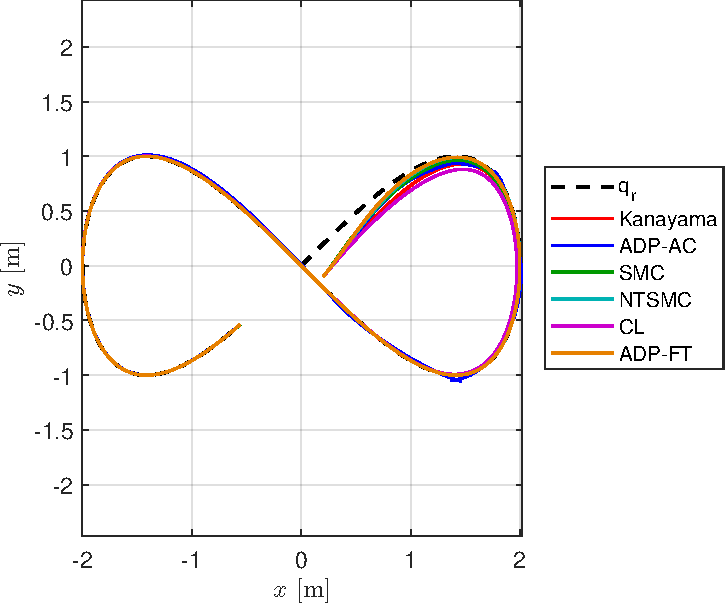
\includegraphics[height=4.45cm]{xy_figure8.pdf}};
    \node[anchor=north west, inner sep=0] (b) at ($(a.north east)+(0.35cm,0)$)
      {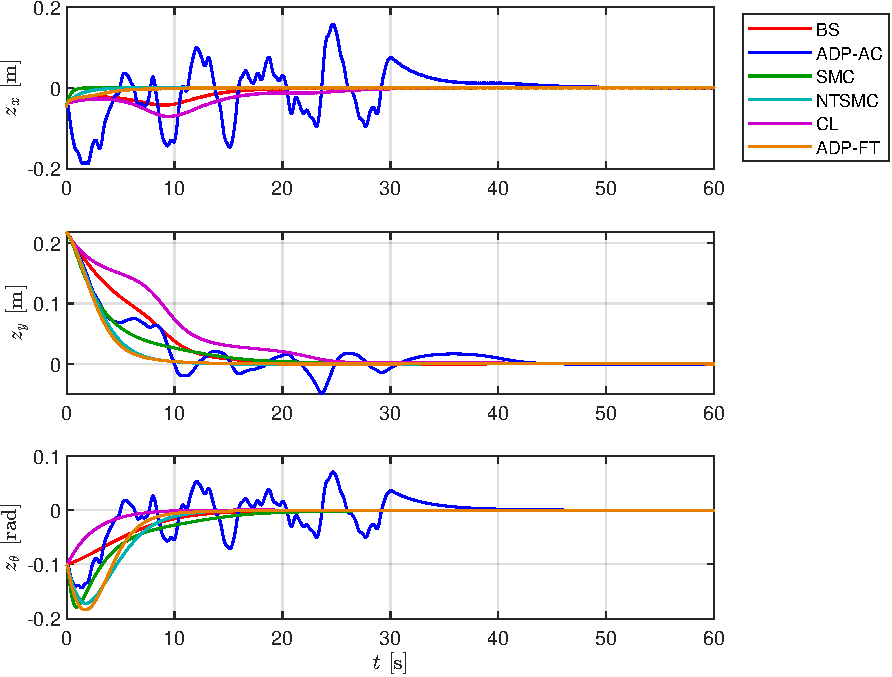
\includegraphics[height=4.45cm]{error_figure8.pdf}};
    \node[anchor=north west, text width=10.4cm, font=\footnotesize, align=left] at ($(a.south west)+(0,-0.2cm)$)
      {Trái: quỹ đạo trên mặt phẳng (nét đứt: tham chiếu $q_r$). Phải: sai số $z_x, z_y, z_\theta$.\\
       Mọi phương pháp đều bám được; ADP-FT về lân cận $0{,}01$\,m sớm nhất ($9{,}2$\,s).};
  \end{tikzpicture}
\end{frame}

\begin{frame}{So sánh năm phương pháp}
  \begin{columns}[T,onlytextwidth]
    \begin{column}{0.52\textwidth}
      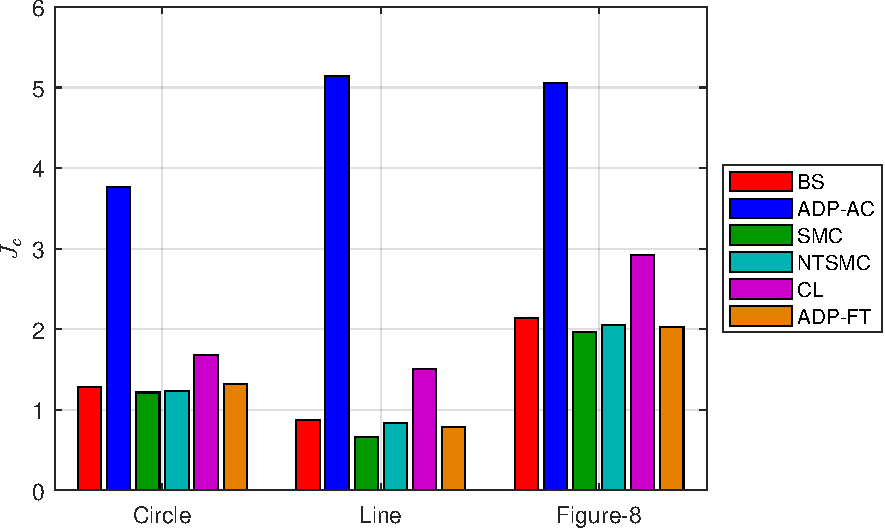
\includegraphics[width=\linewidth]{bar_jc_traj.pdf}\\[1pt]
      \hint{$J_c$ trên ba quỹ đạo: (a) tròn, (b) thẳng, (c) số 8}
    \end{column}
    \begin{column}{0.45\textwidth}
      \footnotesize
      \renewcommand{\arraystretch}{1.15}
      \begin{tabular}{@{}lrr@{}}
        \toprule
        Phương pháp & $\sum J_c$ & $t_{0,01}$ (tròn) \\
        \midrule
        SMC & \textbf{3,837} & 10,1\,s \\
        NTSMC & 4,130 & 9,1\,s \\
        \textbf{ADP-FT} & 4,140 & \textbf{6,0\,s} \\
        Kanayama & 4,290 & 9,9\,s \\
        CL & 6,099 & 31,1\,s \\
        ADP-AC & 13,951 & 37,5\,s \\
        \bottomrule
      \end{tabular}\\[0.2cm]
      ADP-FT ngang NTSMC, kém SMC đã chỉnh $7{,}9\%$; về lân cận $0{,}01$\,m nhanh nhất.\\[0.08cm]
      \hint{Ở hệ số thông dụng, SMC ($4{,}887$) lại kém ADP-FT.}
    \end{column}
  \end{columns}
\end{frame}

\begin{frame}{Độ bền với nhiễu mô-men}
  \begin{columns}[T,onlytextwidth]
    \begin{column}{0.47\textwidth}
      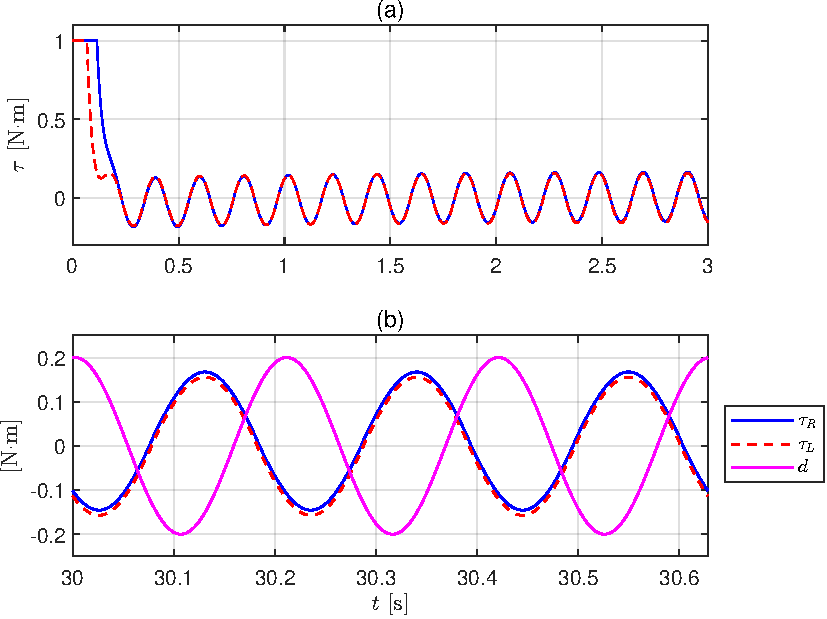
\includegraphics[width=\linewidth]{torque_dist.pdf}\\[1pt]
      \hint{(a) 3\,s đầu: bão hòa khi khởi động; (b) xác lập: mô-men gần như ngược pha với nhiễu $d$}
    \end{column}
    \begin{column}{0.5\textwidth}
      \vspace{0.1cm}
      \stat{≤\,2\%}{thay đổi $J_c$ khi nhiễu tăng $0 \to 60\%\,\tau_{\max}$ (ba dạng: đồng pha, vi sai, độc lập)}\\[0.3cm]
      \stat{21--23\%}{sai số xác lập giảm nhờ số hạng cố định thời gian của vòng 2 (so với luật Fierro \& Lewis)}\\[0.3cm]
      {\footnotesize Sai số xác lập do nhiễu \textbf{như nhau ở mọi luật vòng 1}: kháng nhiễu mô-men là nhiệm vụ của vòng 2.}
    \end{column}
  \end{columns}
\end{frame}

% ================================================================ 5. Ket luan
\section{Kết luận}
\begin{frame}{Kết luận}
  \begin{enumerate}\setlength{\itemsep}{0.22cm}
    \item \textbf{Bộ điều khiển hai vòng theo backstepping} hoạt động trên robot nhận lệnh mô-men, có hàm Lyapunov chung (Định lý 4.1); mô-men chỉ bão hòa lúc khởi động.
    \item \textbf{Khoảng hở kênh ngang} của luật gốc được chỉ ra (Bổ đề 4.1) và khắc phục bằng số hạng ghép -- thành phần quyết định hiệu năng.
    \item \textbf{So sánh công bằng}: ADP-FT ngang NTSMC, kém SMC đã chỉnh $7{,}9\%$, về lân cận $0{,}01$\,m của quỹ đạo nhanh nhất.
    \item \textbf{Độ bền với nhiễu} do vòng 2 quyết định: chi phí đổi không quá $2\%$ với nhiễu tới $60\%\,\tau_{\max}$.
  \end{enumerate}
\end{frame}

\begin{frame}{Hạn chế và hướng phát triển}
  \begin{columns}[T,onlytextwidth]
    \begin{column}{0.48\textwidth}
      {\bfseries\color{hustred}Hạn chế}
      \begin{itemize}\setlength{\itemsep}{0.12cm}\footnotesize
        \item Hội tụ của sai số ngang $z_y$ khi có số hạng ghép mới kiểm chứng bằng mô phỏng.
        \item Lệnh vận tốc bị chặn: hội tụ cố định thời gian không được bảo toàn trên toàn miền.
        \item Việc học trực tuyến của Critic chưa cải thiện so với Critic khởi tạo tốt.
        \item Chưa thực nghiệm trên robot thật.
      \end{itemize}
    \end{column}
    \begin{column}{0.48\textwidth}
      {\bfseries\color{hustred}Hướng phát triển}
      \begin{itemize}\setlength{\itemsep}{0.12cm}\footnotesize
        \item Luật học phù hợp với bộ điều khiển hai vòng.
        \item Hàm Lyapunov kiểu Kanayama cho vòng 1 để chứng minh hội tụ của $z_y$.
        \item Kiểm chứng trên robot vi sai thực.
      \end{itemize}
    \end{column}
  \end{columns}
\end{frame}

% ================================================================ Cam on
{\setbeamertemplate{background}{
\includegraphics[width=\paperwidth,height=\paperheight]{bg_thanks.jpg}}
 \setbeamertemplate{footline}{}
\begin{frame}[plain]
\begin{tikzpicture}[remember picture, overlay]
  \node[align=center] at ($(current page.north)+(0,-3.3cm)$)
    {{\fontsize{26}{30}\selectfont\bfseries\color{hustred}XIN TRÂN TRỌNG CẢM ƠN!}\\[0.45cm]
     {\small\color{muted}Kính mong nhận được ý kiến của Hội đồng}};
\end{tikzpicture}
\end{frame}}

\end{document}
